\documentclass[a4paper, 12pt]{article}
\usepackage{tikz}
\usetikzlibrary{positioning, arrows.meta, fit, calc}
\usepackage{xcolor}
\usepackage{float}
\usepackage{caption}
\usepackage{geometry}
\geometry{margin=1.5cm, landscape}

\definecolor{ehead}{RGB}{28,54,105}
\definecolor{seqgreen}{RGB}{220,245,220}
\definecolor{seqred}{RGB}{252,225,225}

\begin{document}
\pagestyle{empty}

\begin{figure}[H]
\centering
\vspace*{-1cm} % Pull it up slightly to ensure it doesn't overflow the page
{\large\bfseries\sffamily Figure 4: Sequence Diagram --- Complete Pipeline}\\[4pt]
{\normalsize\sffamily End-to-end generation, validation, and persistence flow on a single page.}
\vspace{10pt}

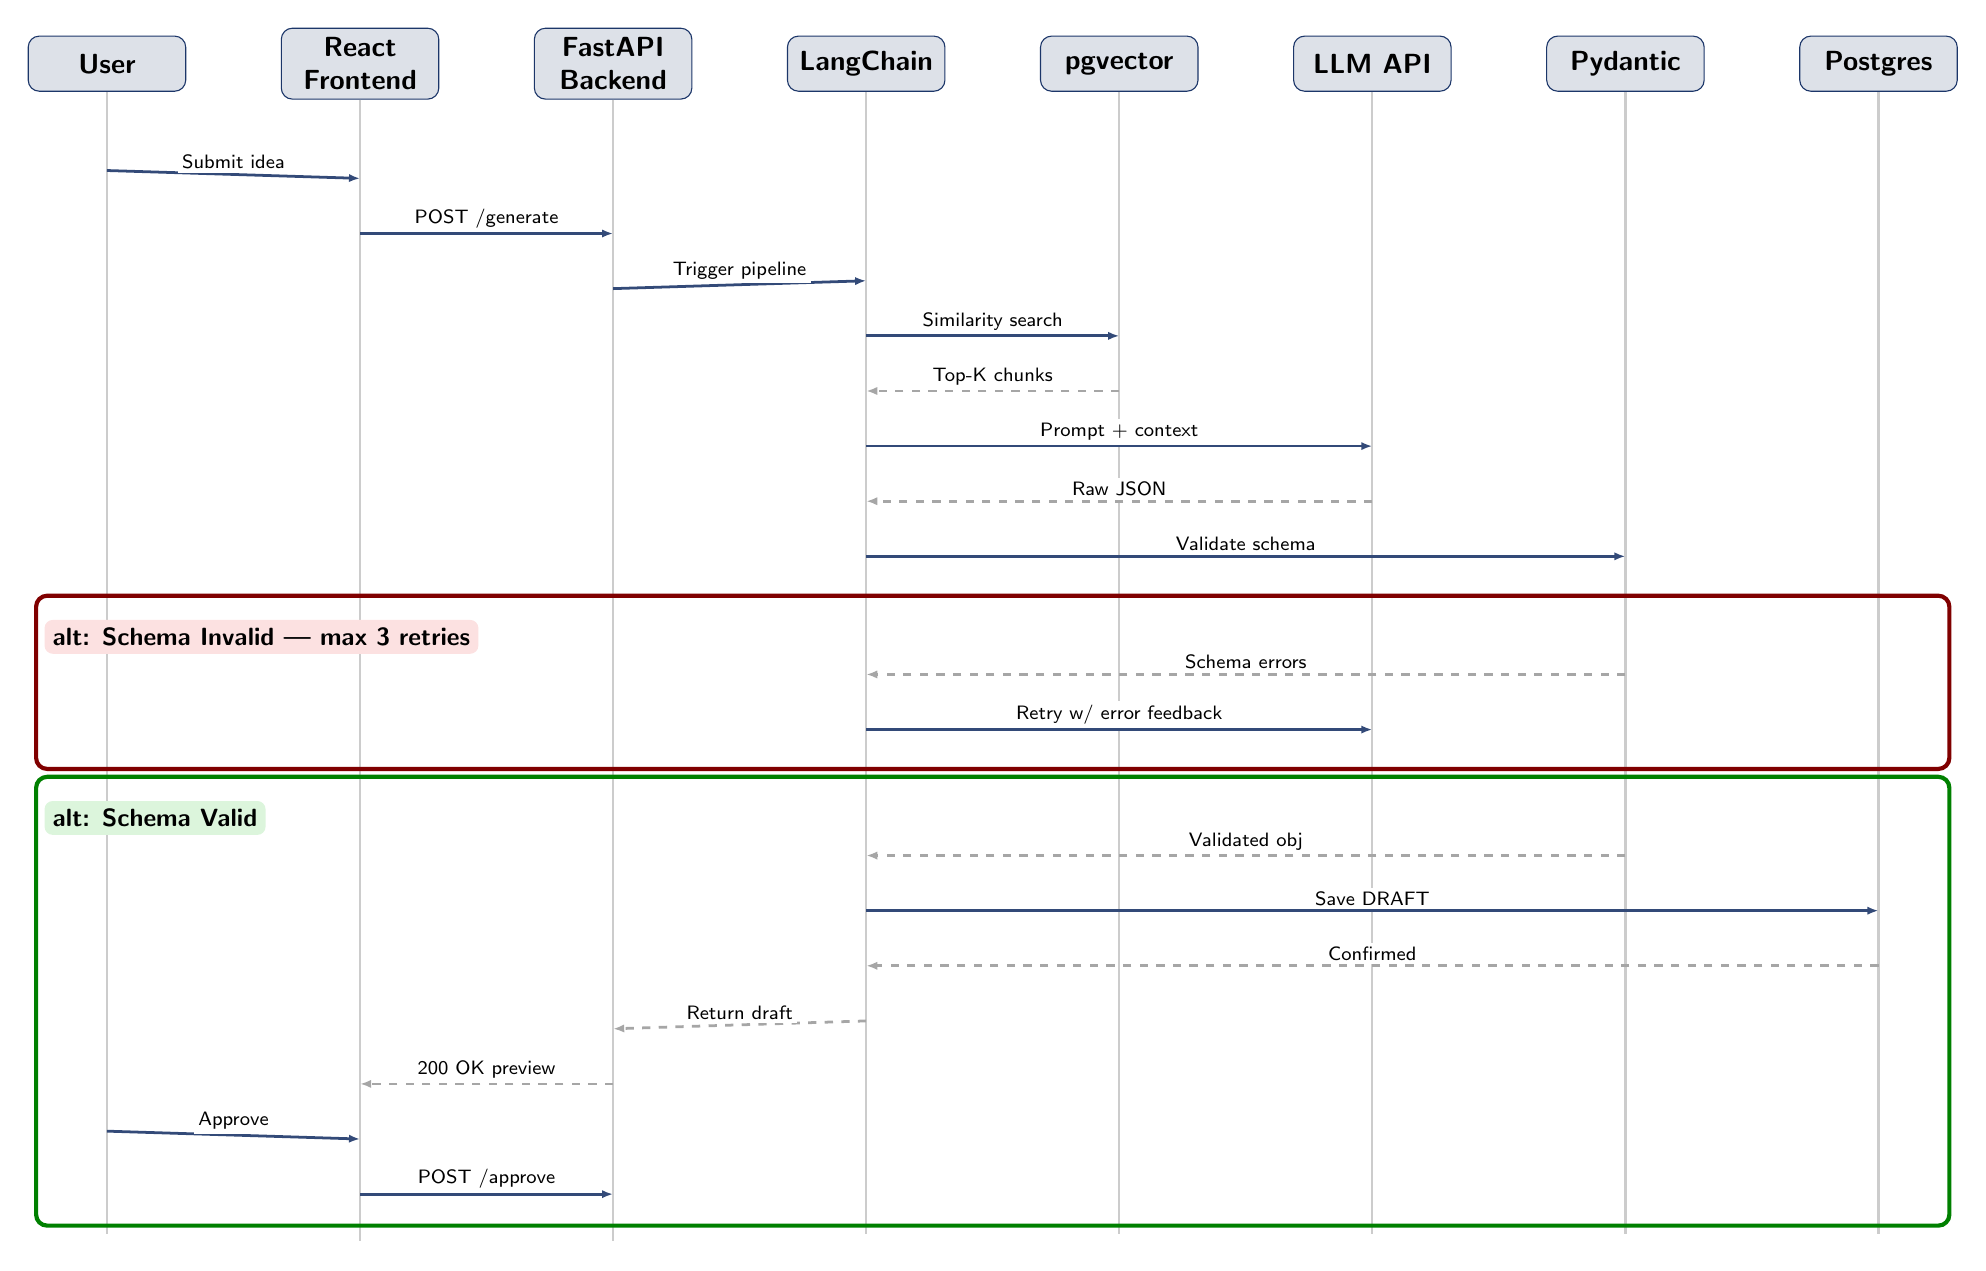
\begin{tikzpicture}[
  actor/.style={rectangle, draw=ehead, fill=ehead!15, rounded corners=4pt,
                minimum width=2cm, minimum height=0.7cm,
                font=\normalsize\bfseries\sffamily, align=center},
  msg/.style={-{Latex[length=4pt, width=3pt]}, line width=1pt, draw=ehead!90},
  ret/.style={-{Latex[length=4pt, width=3pt]}, line width=1pt, draw=gray!70, dashed},
  msglbl/.style={font=\scriptsize\sffamily, fill=white, inner sep=1.5pt},
  blklabel/.style={font=\small\bfseries\sffamily, fill=#1,
                   inner sep=3pt, rounded corners=3pt},
  node distance=1.2cm
]

% ===== ACTOR HEADERS =====
\node[actor] (user) {User};
\node[actor, right=of user] (fe) {React\\Frontend};
\node[actor, right=of fe] (api) {FastAPI\\Backend};
\node[actor, right=of api] (lc) {LangChain};
\node[actor, right=of lc] (rag) {pgvector};
\node[actor, right=of rag] (llm) {LLM API};
\node[actor, right=of llm] (pyd) {Pydantic};
\node[actor, right=of pyd] (db) {Postgres};

% ===== LIFELINES =====
% Reduced from -16 to -14.5 to strictly fit on the first page
\foreach \n in {user,fe,api,lc,rag,llm,pyd,db}{
  \draw[gray!40, line width=0.8pt] (\n.south) -- ++(0,-14.5);
}

% ===== Y POSITIONS (Compressed slightly to fit on 1 page) =====
\def\sa{-1.0}
\def\sb{-1.7}
\def\sc{-2.4}
\def\sd{-3.1}
\def\se{-3.8}
\def\sf{-4.5}
\def\sg{-5.2}
\def\sh{-5.9}

\def\ija{-6.7} % Invalid block start
\def\sj{-7.4}
\def\sk{-8.1}

\def\vja{-9.0} % Valid block start
\def\sl{-9.7}
\def\sm{-10.4}
\def\sn{-11.1}
\def\so{-11.8}
\def\sp{-12.5}
\def\sq{-13.2}
\def\sr{-13.9}

% ===== MESSAGES =====
\draw[msg] ($(user.south)+(0,\sa)$) -- node[msglbl, above]{Submit idea} ($(fe.south)+(0,\sa)$);
\draw[msg] ($(fe.south)+(0,\sb)$) -- node[msglbl, above]{POST /generate} ($(api.south)+(0,\sb)$);
\draw[msg] ($(api.south)+(0,\sc)$) -- node[msglbl, above]{Trigger pipeline} ($(lc.south)+(0,\sc)$);

\draw[msg] ($(lc.south)+(0,\sd)$) -- node[msglbl, above]{Similarity search} ($(rag.south)+(0,\sd)$);
\draw[ret] ($(rag.south)+(0,\se)$) -- node[msglbl, above]{Top-K chunks} ($(lc.south)+(0,\se)$);

\draw[msg] ($(lc.south)+(0,\sf)$) -- node[msglbl, above]{Prompt + context} ($(llm.south)+(0,\sf)$);
\draw[ret] ($(llm.south)+(0,\sg)$) -- node[msglbl, above]{Raw JSON} ($(lc.south)+(0,\sg)$);

\draw[msg] ($(lc.south)+(0,\sh)$) -- node[msglbl, above]{Validate schema} ($(pyd.south)+(0,\sh)$);

% ===== INVALID BLOCK =====
\node[blklabel=seqred, anchor=north west] at ($(user.south)+(-0.8,\ija)$) {alt: Schema Invalid --- max 3 retries};
\draw[red!50!black, line width=1.5pt, rounded corners=4pt]
  ($(user.south)+(-0.9,\ija+0.3)$) rectangle ($(db.south)+(0.9,\sk-0.5)$);

\draw[ret] ($(pyd.south)+(0,\sj)$) -- node[msglbl, above]{Schema errors} ($(lc.south)+(0,\sj)$);
\draw[msg] ($(lc.south)+(0,\sk)$) -- node[msglbl, above]{Retry w/ error feedback} ($(llm.south)+(0,\sk)$);

% ===== VALID BLOCK =====
\node[blklabel=seqgreen, anchor=north west] at ($(user.south)+(-0.8,\vja)$) {alt: Schema Valid};
\draw[green!50!black, line width=1.5pt, rounded corners=4pt]
  ($(user.south)+(-0.9,\vja+0.3)$) rectangle ($(db.south)+(0.9,\sr-0.5)$);

\draw[ret] ($(pyd.south)+(0,\sl)$) -- node[msglbl, above]{Validated obj} ($(lc.south)+(0,\sl)$);
\draw[msg] ($(lc.south)+(0,\sm)$) -- node[msglbl, above]{Save DRAFT} ($(db.south)+(0,\sm)$);
\draw[ret] ($(db.south)+(0,\sn)$) -- node[msglbl, above]{Confirmed} ($(lc.south)+(0,\sn)$);
\draw[ret] ($(lc.south)+(0,\so)$) -- node[msglbl, above]{Return draft} ($(api.south)+(0,\so)$);
\draw[ret] ($(api.south)+(0,\sp)$) -- node[msglbl, above]{200 OK preview} ($(fe.south)+(0,\sp)$);
\draw[msg] ($(user.south)+(0,\sq)$) -- node[msglbl, above]{Approve} ($(fe.south)+(0,\sq)$);
\draw[msg] ($(fe.south)+(0,\sr)$) -- node[msglbl, above]{POST /approve} ($(api.south)+(0,\sr)$);

\end{tikzpicture}
\end{figure}

\end{document}
